\documentclass[journal]{IEEEtran}

\usepackage[]{graphicx}
\usepackage{amsmath}
\usepackage{mathtools}
\usepackage{subfiles}
\usepackage{amssymb}
\usepackage{hyperref}
\usepackage{algorithm}
\usepackage{tikz,tikz-3dplot}
\usepackage{pgfplots}
\usepackage{subcaption}
\usepackage{amsmath}
\usepackage[noend]{algpseudocode}
\usepackage{algorithmicx}
\usepackage{tabularx}

\newcommand{\ignore}[1]{}  % {} empty inside = %% comment
\graphicspath{ {./pics/} }

\ifCLASSINFOpdf
\else
\fi

\hyphenation{op-tical net-works semi-conduc-tor}


\begin{document}
\onecolumn

\title{Heterogenous Multi-Robot Testing and Exploration}

\author{Jackson~Parker}

% The paper headers
\markboth{CSEE 8300, Spring 2019, APRIL 2019}%
{Shell \MakeLowercase{\textit{et al.}}: Bare Demo of IEEEtran.cls for IEEE Journals}



\maketitle


\begin{abstract}
  The Heterogeneous Autonomous Robotic Exploration system (HARE) is meant as a proof
  of concept for cooperative heterogeneous systems that divide tasks based on the
  differentiable capabilities of the robots. This research project ended up down
  an interesting path due to early design choices, leading to the creation of a
  custom ROS package for simple testing of systems like this.
\end{abstract}


%%%%%%%%%%%%%%%%%%%%%%%%%%%%%%%%%%%%%%
\section{Introduction}
%%%%%%%%%%%%%%%%%%%%%%%%%%%%%%%%%%%%%%
\subfile{tex/intro}

%%%%%%%%%%%%%%%%%%%%%%%%%%%%%%%%%%%%%%%%%%%
\section{Methodology}
%%%%%%%%%%%%%%%%%%%%%%%%%%%%%%%%%%%%%%%%%%%
\subfile{tex/methodology}

%%%%%%%%%%%%%%%%%%%%%%%%%%%%%%%%%%%%%%%%%%%
\section{Discussion}
%%%%%%%%%%%%%%%%%%%%%%%%%%%%%%%%%%%%%%%%%%%
\subfile{tex/discussion}

%\section{Appendix}
\subfile{tex/appendix}




\bibliographystyle{IEEEtran}
\bibliography{IEEEabrv,sources} % ftp://tug.ctan.org/pub/tex-archive/macros/latex/contrib/IEEEtran/bibtex/IEEEtran_bst_HOWTO.pdf


\begin{IEEEbiography}[{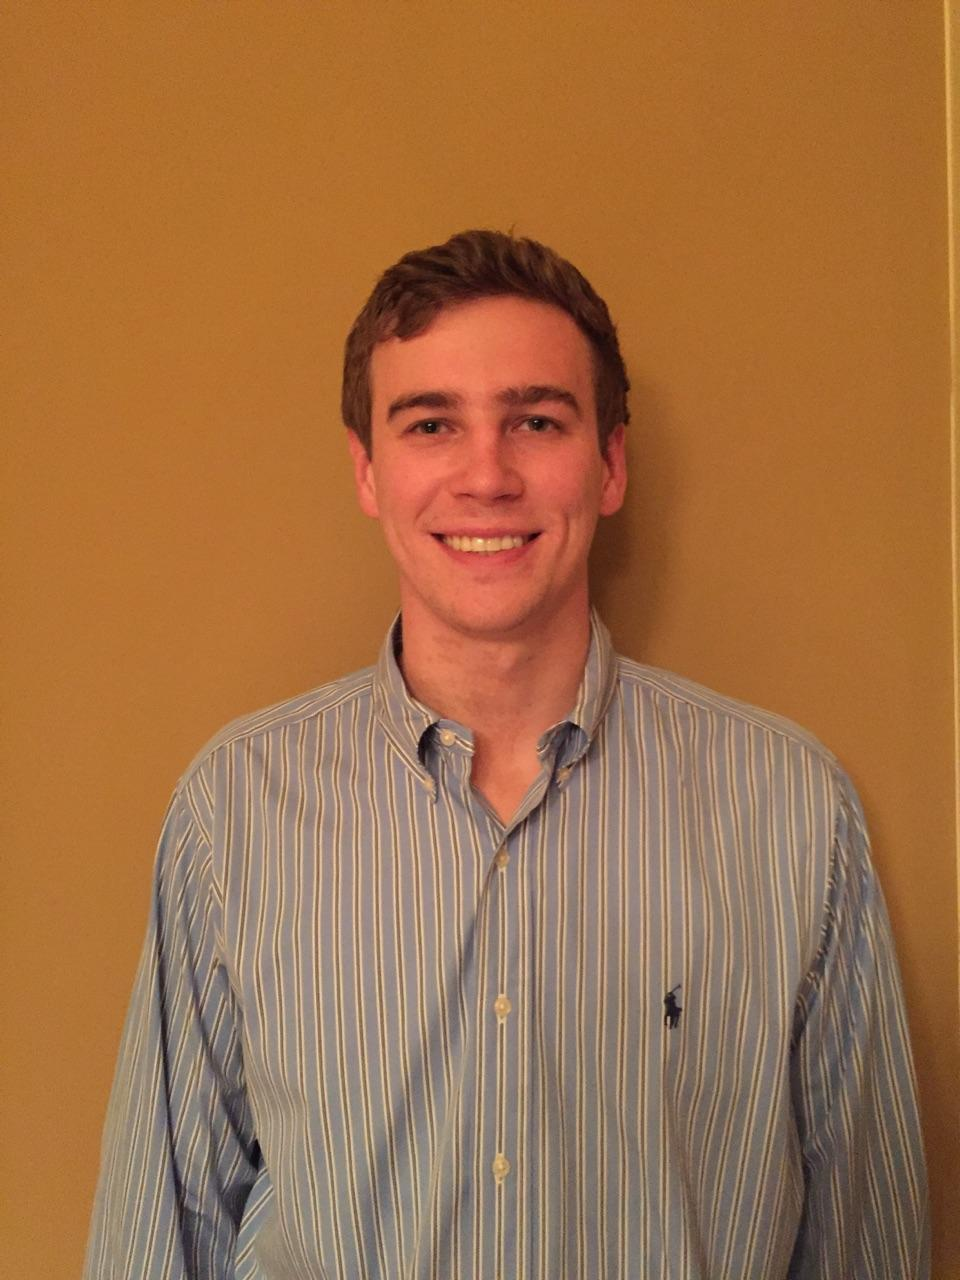
\includegraphics[width=1in,height=1.25in,clip,keepaspectratio]{pics/jackson_parker.jpeg}}]{Jackson Parker}
Currently a Masters Student in the ECE Department at UGA, working as a systems engineer
in the Small Satellite Research Lab
\end{IEEEbiography}



\end{document}
